\parindent=0em
\subsection{Teléfonos móviles}
\noindent

%https://www.aniwaa.com/product/vr-ar/tesseract-holoboard-enterprise-edition/

Los teléfonos móviles son un gran dispositivo ya que combinan \textit{GPS}, cámara, brújula y un acelerómetro, cubriendo así las necesidades de una aplicación de realidad aumentada~\cite{arsmartphones}, además, es un dispositivo muy común entre la población lo cual facilita el desarrollo y expansión de esta realidad. Por otro lado, los teléfonos móviles se pueden utilizar también para realidad mixta utilizando unos cascos en los que se coloca el móvil dentro de estos.\\

Existen distintos \textit{HMD} que se utilizan para estas experiencias de realidad mixta acoplando los móviles a alguna parte de las gafas, como por ejemplo, las \textit{Holoboard Enterprise Edition} de la mano de la empresa \textit{TESSERACT} (figura~\ref{fig:mrandroidTESSERACT}). Este dispositivo es compatible a partir de \textit{Android} 6.0  y como especificaciones técnicas se pueden destacar sus 82º de \textit{FOV}, del inglés Field Of View (hace referencia a la amplitud del campo de visión que ofrece el dispositivo, los seres humanos pueden llegar hasta 180º gracias a los dos ojos), utiliza la tecnología \textit{SLAM} para el \textit{tracking}, posee un controlador \textit{6DoF} y utiliza el \textit{tracking} por sensores \textit{IMU}(del inglés Inertial Measurement Unit), además, permite experiencias colaborativas en la nube.

\begin{figure}[H]
    \centering
    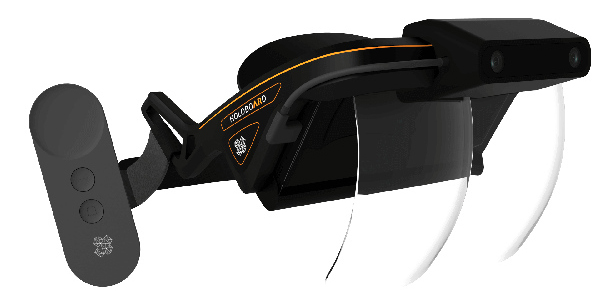
\includegraphics[scale=0.4]{Images/Estado del arte/mrandroid.jpg}
    \caption{
    \textit{Holoboard Enterprise Edition}
    \protect\footnote{\url{https://www.aniwaa.com/product/vr-ar/tesseract-holoboard-enterprise-edition}}
    }
    \label{fig:mrandroidTESSERACT}
\end{figure}

En cambio, si estamos hablando de un dispositivo para utilizar en móviles con \textit{iOS} podemos hablar del casco \textit{Bridge} (figura~\ref{fig:mriosBRIDGE}) de la empresa \textit{Occipital}. Este \textit{HMD} requiere de un componente extra llamado \textit{Occipital Structure Sensor}, el cual, se utiliza para el escaneo 3D del dispositivo.

\begin{figure}[H]
    \centering
    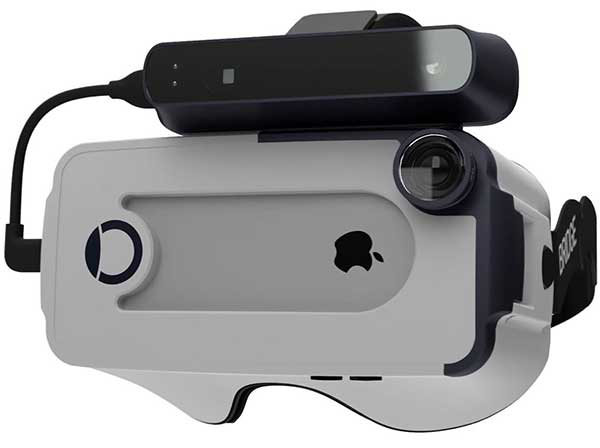
\includegraphics[scale=0.3]{Images/Estado del arte/mrios.jpg}
    \caption{
    \textit{Occipital Bridge}
    \protect\footnote{\url{https://www.aniwaa.com/product/vr-headsets/occipital-bridge/}}
    }
    \label{fig:mriosBRIDGE}
\end{figure}

Las gafas \textit{Bridge} tienen un \textit{FOV} de 120º, un controlador de \textit{6DoF} y destacan por que gracias a estas se puede utilizar aplicaciones de realidad aumentada, realidad mixta y realidad virtual, también, la técnica de \textit{tracking} conocida como \textit{Inside-out}.\\

Pese a que la principal diferencia entre las dos gafas es el sistema operativo para el que están destinadas, se puede observar que los precios son similares y que las gafas destinadas para \textit{iOS} poseen un \textit{FOV} notablemente superior.


\begin{table}[H]
\centering
\renewcommand{\arraystretch}{1.5}
\begin{tabular}{llllll}
\hline
Dispositivo                  & Precio & \textit{DoF} & \textit{FOV} & \textit{SO} & \textit{Tracking} \\
\hline
Holoboard Enterprise Edition & \$399  & 6DoF         & 82º          & Android     & SLAM              \\
Occipital Bridge             & \$349  & 6DoF         & 120º         & iOS         & Inside-out\\\hline       
\end{tabular}
\caption{Comparación entre ambas gafas de \textit{MR} para móviles.}
\label{cuadro:comparacionphonesMR}
\end{table}

